\documentclass[22pt]{article} 
\usepackage{geometry} 
\usepackage{float} 
\usepackage{graphicx}
\usepackage{caption}
\usepackage{subfigure}
\usepackage{amsmath}
\usepackage{array}
\geometry{left=2.0cm,right=2.0cm,top=0.5cm,bottom=0.5cm}
	\author{Mengfan Wang} 
	\title{Optimization Techniques Homework 1} 
\begin{document}
	\maketitle 
	\paragraph{1}
		\subparagraph{a} An infeasible linear programming problem:
		\begin{align}
			min \quad y_1+y_2\\
			s.t. \quad y_1+y_2 & \geq 2\\
					   -y_1 - y_2 & \geq -1\\
					   y_1 & \geq 0\\
					   y_2 & \geq 0
		\end{align}
		\subparagraph{b} A feasible unbounded linear programming problem:
		\begin{align}
			min \quad -y_1-y_2\\
			s.t. \quad y_1+y_2 & \geq 2\\
					   y_1 + y_2 & \geq 1\\
					   y_1 & \geq 0\\
					   y_2 & \geq 0
		\end{align}
		\subparagraph{c} A feasible bounded linear programming problem:
		\begin{align}
			min \quad y_1+y_2\\
			s.t. \quad -y_1-y_2 & \geq -2\\
					   y_1 + y_2 & \geq 1\\
					   y_1 & \geq 0\\
					   y_2 & \geq 0
		\end{align}

	\paragraph{2}Suppose $\mathbf{x}_0$ is a optimal solution for a maximum linear problem, not at one corner but in the constraint set or on one edge. Suppose $z = \mathbf{c^Tx}_0$, which is the maximum value of the objective function. Because the constraint set is a bounded convex set, $\mathbf{x}_0$ can always be represented by a convex combination of some corners. Suppose $\mathbf{x}_0 = \sum\limits_{i=1}^{n}a_i\mathbf{x}_i$, while $\mathbf{x}_1$ to $\mathbf{x}_n$ are corners and $\sum\limits_{i=1}^{n}a_i = 1$. Then we have:
	\begin{equation}
		z = \mathbf{c^Tx}_0 = \mathbf{c^T}(\sum\limits_{i=1}^na_i\mathbf{x}_i) = \sum\limits_{i=1}^na_i\mathbf{c^Tx}_i \leq \sum\limits_{i=1}^na_iz = z
	\end{equation}
	Because the left part of the equation equals to the right part, $\sum\limits_{i=1}^na_i\mathbf{c^Tx}_i = \sum\limits_{i=1}^na_iz$. $\mathbf{c^Tx}_i$ can not be greater than $z$, and thus for all $i$, $\mathbf{c^Tx}_i = z$. In conclusion, all corners which take part in the presentation of $\mathbf{x}_0$ are optimal solutions. 

	This proposition for a minimum linear problem can be proved in a similar way.

	\paragraph{3}
		\subparagraph{Proof of 1}Let the new tableau be denoted with hats on the variables. We are to show $-\hat{c}_j \geq 0$ for all j. For $j = j_0$ we have $-\hat{c}_{j0} = -\frac{-c_{j0}}{a_{i0,j0}}$ still nonnegative, since $a_{i0,j0} < 0$. For $j \not= j_0$, we have 
		\begin{equation}
			-\hat{c}_j = -c_j - \frac{-c_{j0}a_{i0,j}}{a_{i0,j0}}
		\end{equation}
		If $a_{i0,j} \geq 0$, then $-\hat{c}_j \geq -c_j \geq 0$ since $\frac{-c_{j0}a_{i0,j}}{a_{i0,j0}} \leq 0$. If $a_{i0,j} < 0$, then by the pivot rule, $\frac{-c_j}{a_{i0,j}} \leq \frac{-c_{j0}}{a_{i0,j0}}$, $-c_j \geq \frac{-c_{j0}a_{i0,j}}{a_{i0,j0}}$, so that $-\hat{c}_j \geq -c_j + c_j = 0$. In conclusion, after pivoting, the $-\mathbf{c}$ row remains nonnegative.

		\subparagraph{Proof of 2} $\hat{v} = v - \frac{-c_{j0}b_{i0}}{a_{i0,j0}} \leq v$, because $-c_{j0} \geq 0$, $a_{i0,j0} < 0$, and $b_{i0} < 0$. In conclusion, the value of the objective function is never larger than the old.

	\paragraph{4}
		\subparagraph{Proof of 1}This proposition is almost the same as Problem 3.1. Suppose $-c_j \geq 0$, so $j \not= k$. If $j = j_0$, then  $-\hat{c}_{j0} = -\frac{-c_{j0}}{a_{i0,j0}} \geq 0$. If $j \not= j_0$, then
		\begin{equation}
			-\hat{c}_j = -c_j - \frac{-c_{j0}a_{i0,j}}{a_{i0,j0}}
		\end{equation}
		Now $\frac{-c_{j0}}{a_{i0,j0}} \leq 0$. Hence, if $a_{i0,j} \geq 0$, then $-\hat{c}_j \geq -c_j \geq 0$. And if $a_{i0,j} < 0$, then $\frac{-c_j}{a_{i0,j}} \leq \frac{-c_{j0}}{a_{i0,j0}}$, so that $-\hat{c}_j \geq 0$. In conclusion, the nonnegative $-c_j$ stays nonnegative after pivoting.

		\subparagraph{Proof of 2} In my point of view, this proposition should be $-c_k$ gets no smaller, rather than $-c_j$. Some other entries in the $-\mathbf{c}$ row can be smaller. If $k = j_0$, then $-\hat{c}_{k} = -\frac{-c_{k}}{a_{i0,k}} > 0 > -c_k$, because $-c_k < 0$ and $a_{i0,k}>0$. If $k \not= j_0$, then
		\begin{equation}
			-\hat{c}_k = -c_k - \frac{-c_{j0}a_{i0,k}}{a_{i0,j0}} \geq -c_j,
		\end{equation}
		since $\frac{-c_{j0}}{a_{i0,j0}} \leq 0$ and $a_{i0,k} > 0$.

	\paragraph{5} This problem can be changed to a standard maximum problem by multiplying the objective function by -1, which is changed to $max \quad y_1+y_2+y_3$. As a result, the simplex method for standard maximum problem can be used:
		\begin{equation}
		\renewcommand\arraystretch{1.5}
			\begin{matrix}
			\begin{array}{c|ccc|c}
			   & y_1 & y_2 & y_3 &  \\ \hline
			  s_1 & 1 & 2 & 1 & 4 \\ 
			  s_2 & 4 & 2 & 1 & 12 \\
			  s_3 & -1 & 1 & \textcircled{1} & 1 \\ \hline
			  & -1 & -1 & -1 & \\ 
			\end{array}
			\end{matrix}
			 \rightarrow 
			\begin{matrix}
			\begin{array}{c|ccc|c}
			  & y_1 & y_2 & s_3 &  \\ \hline
			  s_1 & \textcircled{2} & 1 & -1 & 3 \\ 
			  s_2 & 5 & 1 & -1 & 11 \\
			  y_3 & -1 & 1 & 1 & 1 \\ \hline
			  & -2 & 0 & 1 & 1 \\
			\end{array}
			\end{matrix}
			\rightarrow 
			\begin{matrix}
			\begin{array}{c|ccc|c}
			  & s_1 & y_2 & s_3 &  \\ \hline
			  y_1 & \frac{1}{2} & \frac{1}{2} & -\frac{1}{2} & \frac{3}{2} \\ 
			  s_2 & -\frac{5}{2} & -\frac{3}{2} & \frac{3}{2} & \frac{7}{2} \\
			  y_3 & \frac{1}{2} & \frac{3}{2} & \frac{1}{2} & \frac{5}{2} \\ \hline
			  & 1 & 1 & 0 & 4 \\
			\end{array}
			\end{matrix}
		\end{equation}
		The optimal solution is $y_1 = \frac{3}{2}, y_2 = 0, y_3= \frac{5}{2}$. The minimum value of the original objective function is -4.

	\paragraph{6}
		\subparagraph{a}The statements corresponding to the simplex algorithm for standard maximization problem should be: 

		1. When $\mathbf{b} \geq 0$, the $\mathbf{b}$ column stays nonnegative, and the value of the objective function of the new tableau is never less than that of the old after pivoting.

		2. When some $b_i$ are negative, the nonnegative $b_i$ stay nonnegative, and $b_k$ has become no smaller after pivoting.

		This phenomenon certainly don't conflict with these statements. However, the simplex algorithm didn't make the value of objective function greater, either. The reason is some $b_i = 0$, and they were chosen as $b_{i0}$ all the time. When $b_{i0} = 0$:
		\begin{align}
			&\hat{b}_{i0} = \frac{b_{i0}}{a_{i0,j0}} = 0\\
			&\hat{b}_i = b_i-\frac{a_{i,j0}b_{i0}}{a_{i0,j0}} = b_i\\
			&\hat{v} = v - \frac{-c_{j0}b_{i0}}{a_{i0,j0}} = v
		\end{align}
		The last column don't be changed at all. With the increasing of iterations, there is a possibility of cycling.


		\subparagraph{b}Add a unit matrix to the right of the $b$-column of the simplex tableau, and an $m$-vector $(c_{n+1}, \cdots, c_{n+m})$, initially \textbf{0}, to the right of the value variable $v$. Modified simplex tableau:
		\begin{figure}[H]
				\centering
				\subfigure{
					\begin{minipage}{14cm}
					\centering 
					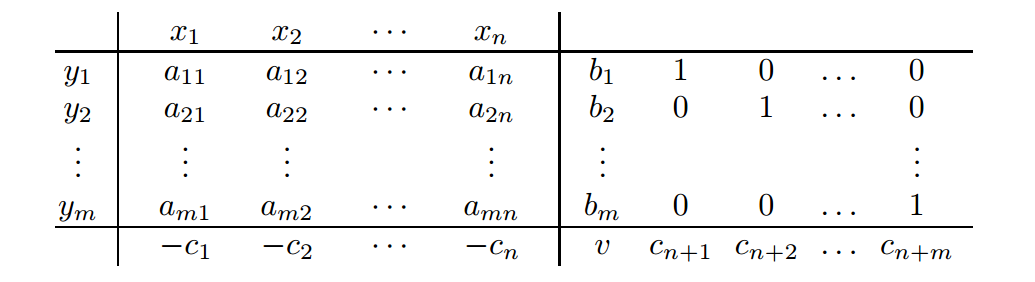
\includegraphics[height=3cm]{Capture.jpg}
					\end{minipage}
				}
			\end{figure}
		 If all $b_i \geq 0$: Choose $c_s < 0$. Among all $r$ such that $a_{r,s} > 0$, pivot about that $a_{r,s}$ to make sure $\frac{\mathbf{b_r}}{a_{r,s}}$ is lexicographically least.

		 If some $b_i$ are negative: Take the first negative $b_i$, say $b_k<0$. Find any negative entry in row k, say $a_{k,s}<0$. Compare $\frac{\mathbf{b}_k}{a_{k,s}}$ and the $\frac{\mathbf{b}_r}{a_{r,s}}$ for which $b_r \geq 0$ and $a_{r,s} > 0$, and choose $r$ for which this ratio is lexicographically least ($r$ may be equal to $k$).

		\subparagraph{c}
		\begin{equation}
		\renewcommand\arraystretch{1.5}
			\begin{matrix}
			\begin{array}{c|cccc|cccc}
			   & x_1 & x_2 & x_3 & x_4 & & & & \\ \hline
			  y_1 & 1 & -2 & -1 & 2 & 0 & 1 & 0 & 0 \\ 
			  y_2 & 2 & -3 & -1 & 1 & 0 & 0 & 1 & 0 \\
			  y_3 & 0 & 0 & \textcircled{1} & 0 & 1 & 0 & 0 &1 \\ \hline
			  & -3 & 5 & -1 & 2 & 0 & 0& 0&0 \\ 
			\end{array}
			\end{matrix}
			\rightarrow
			\begin{matrix}
			\begin{array}{c|cccc|cccc}
			   & x_1 & x_2 & y_3 & x_4 & & & & \\ \hline
			  y_1 & 1 & -2 & 1 & 2 & 1 & 1 & 0 & 1 \\ 
			  y_2 & \textcircled{2} & -3 & 1 & 1 & 1 & 0 & 1 & 1 \\
			  x_3 & 0 & 0 & 1 & 0 & 1 & 0 & 0 &1 \\ \hline
			  & -3 & 5 & 1 & 2 & 1 & 0& 0&1 \\ 
			\end{array}
			\end{matrix}
			\end{equation}
			\begin{equation}
			 \rightarrow 
			 \renewcommand\arraystretch{1.5}
			 \begin{matrix}
			\begin{array}{c|cccc|cccc}
			   & y_2 & x_2 & y_3 & x_4 & & & & \\ \hline
			  y_1 & -\frac{1}{2} & -\frac{1}{2} & \frac{1}{2} & \frac{3}{2} & \frac{1}{2} & 1 & -\frac{1}{2} & \frac{1}{2} \\ 
			  x_1 & \frac{1}{2} & -\frac{3}{2} & \frac{1}{2} & \frac{1}{2} & \frac{1}{2} & 0 & \frac{1}{2} & \frac{1}{2} \\
			  x_3 & 0 & 0 & 1 & 0 & 1 & 0 & 0 &1 \\ \hline
			  & \frac{3}{2} & \frac{1}{2} & \frac{5}{2} & \frac{7}{2} & \frac{5}{2} & 0& \frac{3}{2}&\frac{5}{2} \\ 
			\end{array}
			\end{matrix}
		\end{equation}
		As a result, the optimal solution to the maximum problem is $x_1 = \frac{1}{2}, x_2= 0, x_3 = 1, x_4 =0$. The maximum value is $\frac{5}{2}$.
\end{document}